\documentclass[UKenglish]{beamer}
\usepackage{pres_preamble}
\usetheme{UiB}


%----------------------------------------------------------------------------------------
%	TITLE PAGE
%----------------------------------------------------------------------------------------

\title{Lorentzian Geometry and Topological Electromagnetism}

\author{Colin Roberts}
\setbeamercolor{title}{fg=white} 
\setbeamercolor{subtitle}{fg=white} 


%----------------------------------------------------------------------------------------
%	PRESENTATION SLIDES
%----------------------------------------------------------------------------------------

\begin{document}

%----------------------------------------------------------------------------------------
%  Thanks and funding
%----------------------------------------------------------------------------------------

\begin{frame}{}
    Thanks and funding
    \begin{figure}[h]
    
\includegraphics[scale=.05]{figures/NASA_logo.png}
    \end{figure}
\end{frame}


%----------------------------------------------------------------------------------------
\section{Introduction}
%----------------------------------------------------------------------------------------



\begin{frame}{Outline}
\vfill
\begin{enumerate}
    \item Intro Lorentzian geometry
    \item Poincar\'e group $\A(1,3)$ and its Lie algebra $\alg(1,3)$
    \item de Rham (Co)homology
    \item Topological electromagnetism
\end{enumerate}
\vfill
\end{frame}

\begin{frame}{Motivation}
plasmas and what not, robotic motion, computer graphics, PDEs, inverse problems
\end{frame}

\begin{frame}{Maxwell's Equations}
    \begin{columns}[c] 

    \column{.45\textwidth}
    
    \begin{center} \textbf{Gauss's Laws}
    
    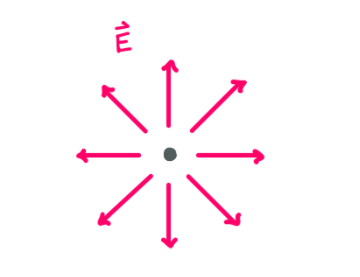
\includegraphics[scale=.4]{figures/gauss_i.png}
    
    \vspace{-10mm}
    
    \small
    $$ \grad\cdot \blade{E} = \rho $$
    
    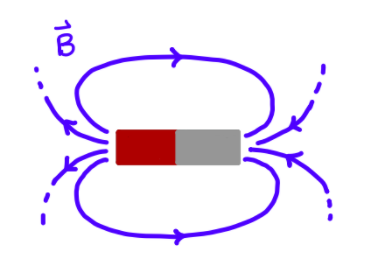
\includegraphics[scale=.4]{figures/gauss_ii.png}
    
    \vspace{-10mm}
    
    $$ \grad \cdot \blade{B} = 0 $$
    
    \end{center}
    
    \column{.45\textwidth}
    
    \begin{center}
    
    \textbf{Ampere's Law}
    
    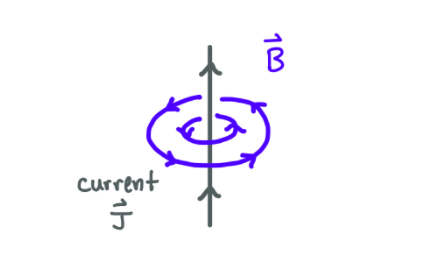
\includegraphics[scale=.4]{figures/ampere.png}
    
    \vspace{-10mm}
    
    \small
    $$ \grad \times \blade{B} - \frac{\partial \blade{E}}{\partial t} = \blade{J} $$
    
    \normalsize
    
    \textbf{Faraday's Law}
    
    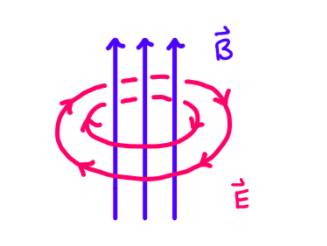
\includegraphics[scale=.4]{figures/faraday.png}
    
    \vspace{-10mm}
    
    \small
    $$ \blade{\nabla} \times \blade{E} + \frac{\partial \blade{B}}{\partial t} = 0 $$ 
    \normalsize
    
    \end{center}
   
    
    \end{columns}
    
    
\end{frame}

%----------------------------------------------------------------------------------------
\section{Lorentzian Geometry}
%----------------------------------------------------------------------------------------

\begin{frame}{Geometry through algebra}
\vfill
\begin{itemize}
	\item Take a vector space $V$ with a quadratic form $Q(-)$
	\item Create the \boldgreen{Clifford algebra} $C\ell(V,Q)$ from the tensor algebra
	\item Elements of $C\ell(V,Q)$ are \boldgreen{multivectors} of grade 0 (scalars) up to grade $n$ (pseudoscalars)
\end{itemize}
\vfill
\end{frame}

\begin{frame}{Euclidean space}
\vfill
Take $\R^n$ with Euclidean norm $|-|$ and an orthonormal basis $\blade{e}_i$.
\begin{itemize}
	\item We have the product in $\G_n\coloneqq C\ell(\R^n,|-|)$ by
	\[
	\blade{e}_i \blade{e}_j = \underbrace{\blade{e}_i \cdot \blade{e_j}}_{\textrm{scalar}} + \underbrace{\blade{e}_i \wedge \blade{e}_j}_{\textrm{bivector}}
	\]
	\item $\delta_{ij}=\blade{e}_i\cdot \blade{e}_j$ are the values of the Euclidean inner product on this basis.
\end{itemize}
\vfill
\end{frame}

\begin{frame}{$\R^3$}
\vfill
Given $\blade{a},\blade{b}\in \G_3$ bivector $\blade{a}\wedge \blade{b}$ represents an oriented plane
	\begin{figure}[H]
		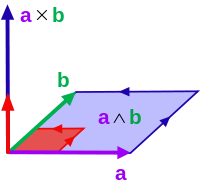
\includegraphics[width=.3\textwidth]{figures/bivector.png}
	\end{figure}
and the perpendicular or \boldgreen{dual} $(\blade{a}\wedge \blade{b})^\perp = \blade{a}\times \blade{b}$.
\vfill
\end{frame}

\begin{frame}{Lorentzian space}
\vfill
Instead, take $\R^4$ with basis $\blade{e}_0,\cdots,\blade{e}_3$ so that
\begin{itemize}
	\item $\blade{e}_0^2 = -1$ (temporal)
	\item $\blade{e}_i^2 = +1$ for $i=1,2,3$ (spatial)
	\item $\blade{e}_\mu \cdot \blade{e}_\nu = 0$ if $\mu \neq \nu$ (orthogonal)
	\item Build $\G_{1,3}$ from these definitions.
\end{itemize}
\vfill
\end{frame}

\begin{frame}{Space Oddity}
\vfill
\center
There exist \boldgreen{null vectors} $\blade{c}$ so that $\blade{c}\cdot \blade{c} = 0$.
\vfill
\end{frame}

\begin{frame}{}
\vfill
\centering Level sets $\blade{p}\cdot \blade{p} = \textrm{constant}$ yield foliations
\vspace*{.5cm}
\begin{columns}[c]
\column{.45\textwidth}
~~~~~~~~~~~~~~~~~~~ Euclidean 

\column{.45 \textwidth}
~~~~~~~Lorentzian
\end{columns}
\begin{center}
    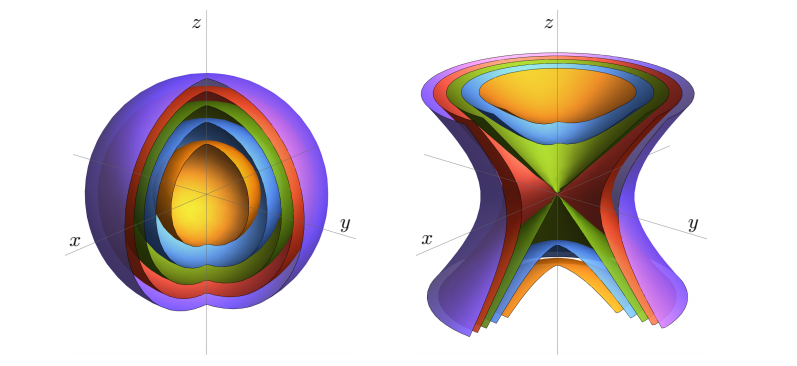
\includegraphics[scale=.5]{figures/foliations2.png}
\end{center}
\vfill   
\end{frame}

\begin{frame}{Question}
    \vfill
    \center
    What are the symmetries of Euclidean space?
    \vfill
\end{frame}

\begin{frame}{Question}
    \vfill
    \center
    What are the symmetries of \boldgreen{Lorentzian} space?
    \vfill
\end{frame}


%----------------------------------------------------------------------------------------
\section{Poincar\'e Group}
%----------------------------------------------------------------------------------------

\begin{frame}{}
\vfill
One way to study geometry is through symmetries of the space.
\vfill
\end{frame}

\begin{frame}{}
\vfill
Want to see what deformations preserve the algebraic structure $\G_n$
\begin{itemize}
	\item Rotations and reflections via the orthogonal group $\mathrm{O}(n)$ and special orthogonal group $\mathrm{SO}(n)$.
	\item Translations (if we keep track of base points) via the group $\R^n$.
	\item These symmetries combine to form \boldgreen{Euclidean group} $\mathrm{E}(n) = \R^n \rtimes \mathrm{O}(n)$ and \boldgreen{special Euclidean group} $\mathrm{SE}(n)=\R^n \rtimes \mathrm{SO}(n)$
\end{itemize}
\vfill
\end{frame}

\begin{frame}{}
\vfill
\begin{itemize}
	\item Given a unit vector $\blade{n}$ and multivector $A$, we have 
	\[
	\blade{n} A \blade{n}^\dagger
	\]
	 reflects $A$ about the hyperplane perpendicular to $\blade{n}$
	\item Given another unit vector $\blade{m}$, 
	\[
	\blade{nm}A(\blade{nm})^\dagger = \blade{nm}A \blade{mn}
	\]
	 yields a rotation in the plane defined by $\blade{n}\wedge \blade{m}$.
\end{itemize}
\vfill
\end{frame}

\begin{frame}{Pin and Spin}
\vfill
\begin{itemize}
	\item Unit vectors generate the group $\blade{n}\in \mathrm{Pin}(n)$ and define a an element $\mathsf{T}\in \mathrm{O}(n)$ by
	\[
	\mathsf{T}(\blade{v}) = \blade{n} \blade{v} \blade{n}^\dagger
	\]
	so the mapping $\blade{n}\mapsto \mathsf{T}$ is 2-to-1.
	\item Likewise, $\blade{nm} \in \mathrm{Spin}(n)$ defines $\mathsf{R} \in \mathrm{SO}(n)$ by
	\[
	\mathsf{R}(\blade{v}) = \blade{nm}\blade{v}(\blade{nm})^\dagger.
	\]
\end{itemize}
\vfill
\end{frame}

\begin{frame}{}
\vfill
\centering Both $\sping(n)$ and $\mathrm{Pin}(n)$ lead to motion on the level sets
\begin{figure}[H]
\centering
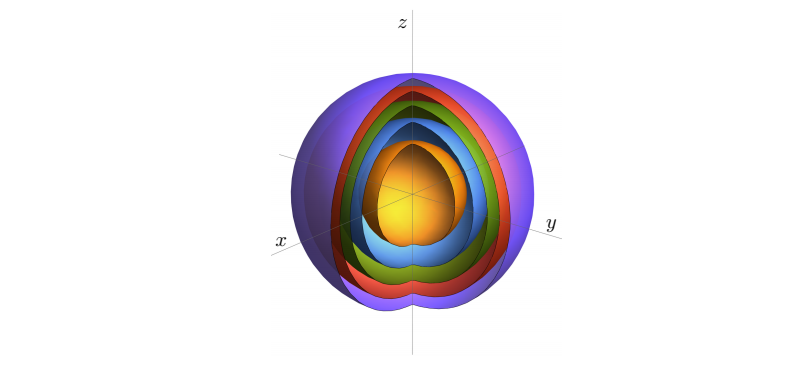
\includegraphics[width=.8\textwidth]{figures/euclidean.png}
\end{figure}
\end{frame}

\begin{frame}{}
\vfill
Hence, we can take $\R^n \rtimes \sping(n)$ to be the rigid symmetries of Euclidean space.
\begin{figure}[H]
\centering
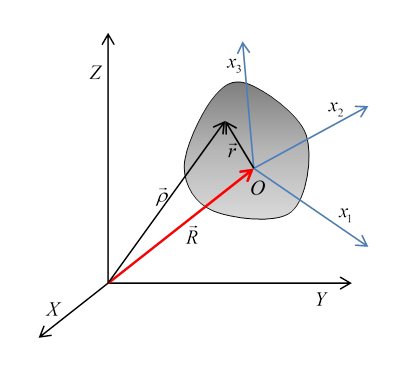
\includegraphics[width=.5\textwidth]{figures/rigid_body.png}
\end{figure} 
\vfill
\end{frame}

\begin{frame}{}
\vfill
\centering Define $\sping(1,3)$ and $\mathrm{Pin}(1,3)$ analogously to see motion on the Lorentzian level sets
\begin{figure}[H]
\centering
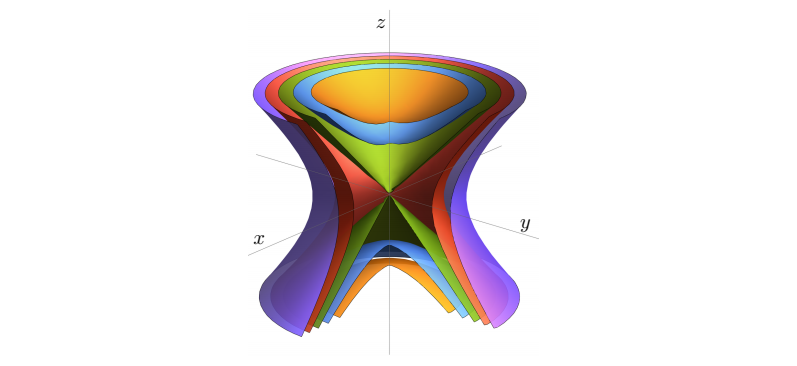
\includegraphics[width=.8\textwidth]{figures/lorentzian.png}
\end{figure}
\end{frame}

\begin{frame}{Relativity}
\vfill
\begin{itemize}
	\item One sheeted hyperboloids are inaccessible regions of space (often called \boldgreen{spacelike})
	\item Two sheeted hyperboloids represent past and future directions (often called \boldgreen{timelike})
	\item Cone consists of all null vectors $\blade{c}\cdot \blade{c} = 0$ which represents \boldgreen{light}.
	\item A particle with rest mass $m$ has 4-momentum $m\blade{v}$ and $\blade{v}\cdot \blade{v}=-1$
	\item The future hyperboloids are foliated by mass.
\end{itemize}
\begin{figure}[H]
\centering
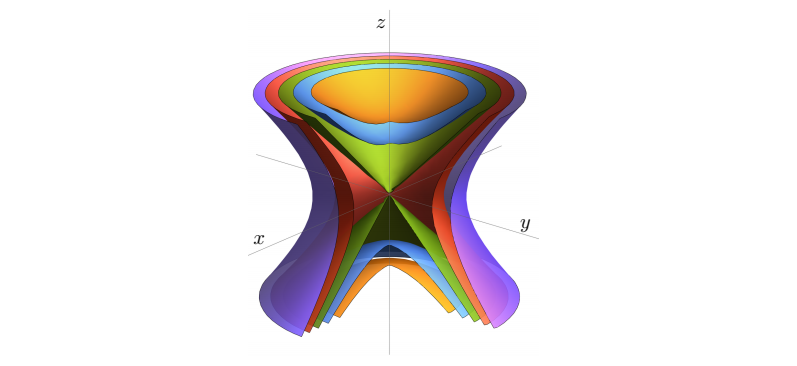
\includegraphics[width=.8\textwidth]{figures/lorentzian.png}
\end{figure}
\vfill
\end{frame}

\begin{frame}{}
\vfill
\begin{itemize}
	\item Motion of a relativistic particle is a curve $\gamma$ in the \boldgreen{Poincar\'e group}
\[
\A(1,3) = \R^{1,3}\rtimes \sping^+(1,3)
\]

        \item Since mass is preserved
        \[
            \grad ({\blade{v}} \cdot {\blade{v}}) = 0 ~\implies~ \nabla_{\blade{v}} {\blade{v}} =  {\blade{v}}\cdot \underbrace{(\grad \wedge {\blade{v}})}_{\textrm{vorticity }\omega}
        \]
        \item Optimal transport of 4-velocity is given by projection onto the vorticity plane
        \begin{figure}
            \centering
            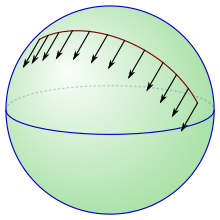
\includegraphics[width=.2\textwidth]{figures/parallel_transport.png}
        \end{figure}
        \end{itemize}
\vfill
\end{frame}



%----------------------------------------------------------------------------------------
\section{de Rham (Co)homology}
%----------------------------------------------------------------------------------------


\begin{frame}{de Rham (Co)homology}
\vfill
\begin{itemize}
    \item Given a manifold $M$, we have the exterior algebra of (compactly supported) forms $\Omega(M)$.
    \begin{itemize} 
        \item de Rham cochain complex is built with the exterior derivative $d$.
        \item de Rham cohomology ring is
        \[
            H^\bullet_{dR}(M) = \bigwedge_{k \in \mathbb{N}} H^k_{dR} = \bigwedge_{k \in \mathbb{N}} \ker d_k ~/~ \im d_{k-1}.
        \]
    \end{itemize}
    \item The dual space $\Omega^*(M)$ is the space of currents $T\colon \Omega(M) \to \R$.
    \begin{itemize}
        \item de Rham chain complex is built with boundary operator $\partial$
        \[
            \partial T[\alpha] = T[d \alpha].
        \]
        \item de Rham homology group is
        \[
            H_\bullet^{dR} = \bigoplus_{k\in \mathbb{N}} H_k^{dR} \coloneqq \bigoplus_{k\in \mathbb{N}} \ker \partial_k ~/~ \im \partial_{k+1}. 
        \]
    \end{itemize}
\end{itemize}
\vfill
\end{frame}

\begin{frame}{Multivector Equivalents of Forms}
\vfill
Given a Riemannian manifold $(M,g)$, take the Clifford algebra bundle $\G(M)$ whose sections are multivector fields.
\begin{itemize}
    \item A $k$-form $\alpha_k$ has a multivector equivalent $A_k$ by
    \[
    \alpha_k = A_k \cdot dX_k.
    \] 
    \begin{itemize}
        \item $d\alpha_k \mapsto \grad \wedge A_k$.
        \item $\delta \alpha_k \mapsto \grad \cdot A_k$.
    \end{itemize}
    \item de Rham cohomology: $H^\bullet_{dR}(M) \cong \bigoplus_{n\in \mathbb{N}} \ker \grad \wedge_k ~/~ \im \grad \wedge_{k+1}$.
    \item de Rham homology: $H_\bullet^{dR} = \bigoplus_{k\in \mathbb{N}} \ker \grad\cdot_k ~/~ \im \grad\cdot_{k+1}$. 
\end{itemize}
\vfill
\end{frame}

\begin{frame}{Multivector Equivalents of Currents}
\vfill
We have the Riemannian volume form $\mu$ and the bilinear pairing of multivectors $(-,-)$
\begin{itemize}
    \item We can take a $k$-current by
    \[
    T[-] = \int_M (T_k,-)\mu.
    \]
    and for a $k$-chain $K$ we have the $k$-current $\delta_K$
    \[
    \delta_K[-] = \int_K \mu_K = \int_M (\blade{I}_K,-)\mu.
    \]
    \item The boundary operator acts accordingly
    \[
    \partial T[\alpha_{k-1}] = T[d\alpha_{k-1}] = \int_M(T_k,\grad \wedge A_{k-1})\mu = \int_M (\grad \cdot T_k,A_{k-1})\mu
    \]
    and by Stokes' theorem
    \[
    \partial \delta_K[\alpha_{k-1}]= \int_{\partial K} \alpha_{k-1}.
    \]
\end{itemize}
\vfill
\end{frame}

\begin{frame}{Useful Theorems}
\vfill

    \begin{theorem}[de Rham's Theorem]
        The singular (co)homology over $\R$ is isomorphic to the de Rham (co)homology.
    \end{theorem}
    \begin{theorem}[Poincar\'e Duality]
        We have $H_k\cong H^{n-k}$ by the dual $\perp$. %this is true for forms with compact support
    \end{theorem}
    \begin{theorem}
        The cap product is given by $\rfloor\colon H^\ell(M) \times H_k(M)\to H_{k-\ell}(M)$.
    \end{theorem}

\vfill
\end{frame}

%----------------------------------------------------------------------------------------
\section{Topological Electromagnetism}
%----------------------------------------------------------------------------------------

\begin{frame}{Axioms}
\vfill
There are four physical postulates for electromagnetism that we write as topological axioms.    
    \begin{itemize}
    \item{\bf{Axiom 1.}} \emph{Conservation of charge:} Current density $\blade{J}_3$ must flow through boundaries of regions $N^4$ so
    \[
    0=\int_{\partial N^4} \blade{J}_3\cdot dX_3=\int_{N^4} (\grad \wedge \blade{J}_3) \cdot dX_4
    \]
    so $\blade{J}_3$ is closed. Hence, for a co-closed 3-current $\delta_{N^3}$  we have $\delta_{N^3}[j_3]=0$ and which implies the magnetic excitation $H$ is the potential $\grad \wedge H=\blade{J}_3$ or dually $\blade{J}=\blade{J}_3^\perp = \grad \cdot H^\perp$ defines a homology class.
    \item{\bf{Axiom 2.}} \emph{Conservation of flux:} The electromagnetic field $F$ defines a cohomology class in $H^2(M)$ by taking a co-closed 2-current $N^2$ and noting
    \[
    \int_{N^2} F \cdot dX_2 = 0 
    \]
    implies $\grad \wedge F=0$.
\end{itemize}
\vfill
\end{frame}

\begin{frame}{Axioms}
\vfill
    \begin{itemize}
    \item{\bf{Axiom 3.}} \emph{Constitutive law:} We relate the excitation $H$ with the field $F$. The simplest case is the linear case given by $F=H^\perp$ which yields the Maxwell equations $\grad F = \blade{J}$ or, in their more recognizable relativistic form
    \begin{align*}
        \grad \wedge F &= 0 && \textrm{(homogeneous)}\\
        \grad \cdot F &= \blade{J} && \textrm{(inhomogeneous)}
    \end{align*}
    The homogeneous equations are Gauss's law for magnetism and Faraday's law whereas the inhomogeneous are Gauss's law for electricity and Ampere's law.
    \item{\bf{Axiom 4.}} \emph{Lorentz force:} The motion of a particle with 4-velocity $\blade{v}$ in a field $F$ is
    \[
    \nabla_{\blade{v}}\blade{v} = \frac{q}{m} \blade{v} \cdot F.
    \]
\end{itemize}
\vfill
\end{frame}

\begin{frame}{Faraday Transport}
    \vfill
    \begin{itemize}
        \item For a charged particle, we have the Lorentz force law $\nabla_{\blade{v}}\blade{v} = \frac{1}{2} \blade{v}\cdot F$
        \item In terms of a proper time parameterization $\frac{d\blade{v}}{d\tau} = \frac{1}{2} \blade{v} \cdot F(\gamma(\tau))$.
    \end{itemize}
    \begin{figure}
        \centering
        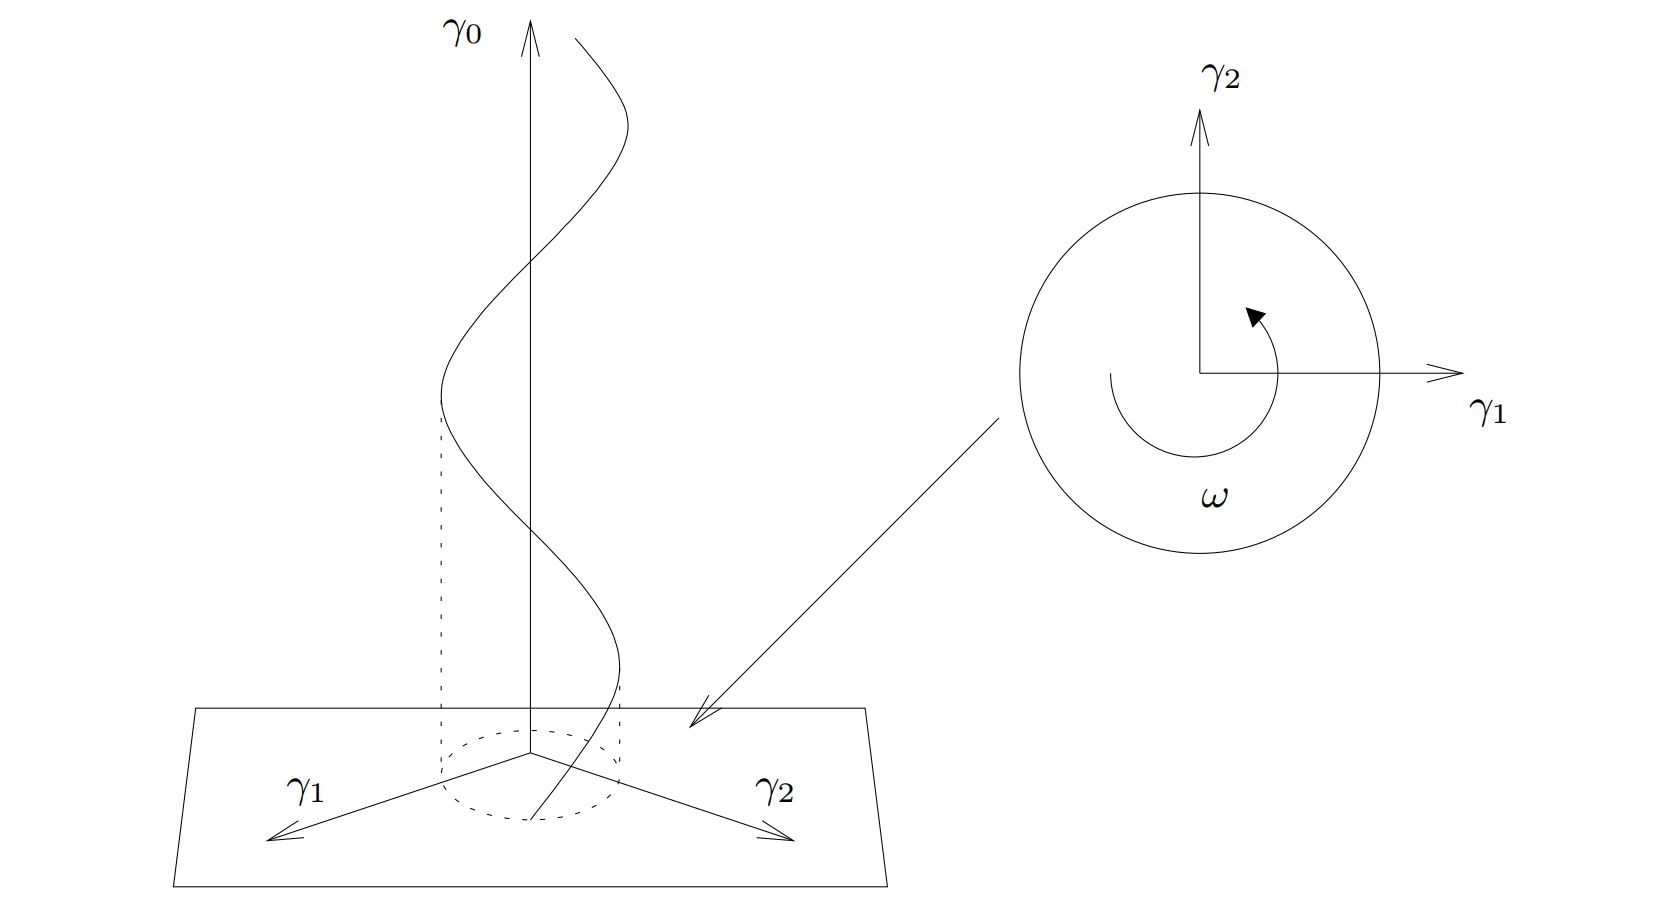
\includegraphics[width=.65\textwidth]{figures/helical_path.png}
    \end{figure}
    \vfill
\end{frame}

\end{document}

%
%

%\section{Plasma Fluids}
%

%
%\begin{frame}{Classical Fluid Quantities}
%\vfill
%    \begin{itemize}
%        \item Vorticity $\blade{\omega}$ represents rotational fluid motion in a plane
%        \begin{figure}
%    \centering
%    \begin{subfigure}[b]{0.15\textwidth}
%        \centering
%        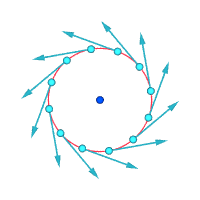
\includegraphics[width=\textwidth]{figures/Vorticity_Figure_01_c.png}
%    \end{subfigure}
%    \hspace*{3cm}
%    \begin{subfigure}[b]{0.15\textwidth}
%        \centering
%        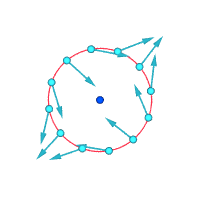
\includegraphics[width=\textwidth]{figures/Vorticity_Figure_02_c.png}
%    \end{subfigure}
%    \end{figure}
%        \item In general, the product of velocity with vorticity decomposes
%        \[
%        \blade{v}\blade{\omega} = \underbrace{\blade{v}\cdot \blade{\omega}}_{\textrm{transport}}+\underbrace{\blade{v}\wedge\blade{\omega}}_{\textrm{helicity}}
%        \]
%            
%        \begin{figure}
%            \centering
%            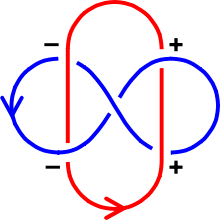
\includegraphics[width=0.15\textwidth]{figures/gauss_linking.png}
%        \end{figure}
%    \end{itemize}
%
%\vfill    
%\end{frame}
%
%%%%%%%%%%%%%%%%%%%%%%%%%%%%%%%%%%%%%%%%%%%%%%%%%%
%

%
%\begin{frame}{Spinor Equations}
%    \vfill
%
%    \begin{itemize}
%        \item Since $\blade{v}\cdot\blade{v}$ is constant, velocity at any $\tau$ is given by time varying isometries
%    \[
%    \blade{v}(\tau)=\mathsf{R}_\tau(\blade{v}_0)
%    \]
%    \item Since $R \in \sping(1,3)$ induces $\mathsf{R}(\blade{v}_0)=R\blade{v}_0 R^\dagger$, particle configuration is a curve in the Lie group $\R^{1,3}\rtimes \sping^+(1,3)$ with Lie algebra $\R^{1,3}\rtimes \spina(1,3)$.
%        \begin{figure}
%        \centering
%        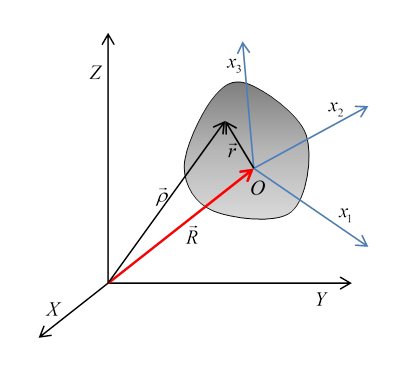
\includegraphics[width=.32\textwidth]{figures/rigid_body.png}
%    \end{figure}
%    \item Fermi-Faraday transport of a spinor is given by $\frac{dR}{d\tau} = FR$
%    \end{itemize}
%    \vfill
%\end{frame}
%
%\begin{frame}{Plasma Fluid}
%    \vfill
%    
%    \begin{itemize}
%        \item Let $m,q\colon N^4 \to \R$ be the mass and charge field and $\blade{v} \in \mathfrak{X}(M)$
%        \item Then the current $\blade{J}=q\blade{v}$
%        \item If we allow mass to flow separately from the velocity 
%        \[
%        \boxed{m\nabla_{\blade{v}}\blade{v} + (\nabla_{\blade{v}}m)\blade{v} = q\blade{v} \cdot \blade{F}}
%        \]
%        \item Assume our axioms of EM so $\grad \cdot \blade{J}=0$ and the constraint that charge to mass is constant yields
%        \[
%        \boxed{\grad \cdot \blade{v} = 0}
%        \]
%        \item Maxwell's equations hold
%        \[
%        \boxed{\grad F = \blade{J}}
%        \]
%    \end{itemize}
%    \vfill
%\end{frame}
%